\chapter{Results}
\label{ch:results}
%
\par As discussed in \S\ref{sec:modeling} and \S\ref{sec:forward_modeling}, hydrodynamic loop models are an invaluable tool for constraining heating properties in the solar corona. In particular, this thesis has focused on developing an efficient two-fluid hydrodynamic model, EBTEL-2fl (see \S\ref{subsec:two_fluid_ebtel}), to study the effect of various heating parameters on the emission measure in active region cores. The 0D nature and consequentially short run times of the EBTEL-2fl code allow for the exploration of a large parameter space. This thesis has used the newly-developed EBTEL-2fl code to examine the effects of varying heating frequency, loop length, heating amplitude power-law distribution index, and preferrentially heated species on the emission measure and the resulting hotward and coolward emission measure slopes (see \S\ref{subsec:scaling}). Altogether, this amounts to a $20\times3\times3\times3$ parameter space for electron and ion heating as well as the single-fluid case. 
%
\par Each EBTEL-2fl run has a simulation time of 80,000 s, with initial conditions determined via static loop solutions (see \ref{subsec:static_v_dynamic}). Flux-limiting (see Eqs. \ref{eq:free_stream_limit} and \ref{eq:flux_limited}) is used so as to more accurately model cooling by thermal conduction in the early heating phase. The Raymond-Klimchuk power-law loss function (see Eq. \hl{RAD LOSS EQ HERE}) is used to model the volumetric radiative losses. In \S\ref{sec:heating_funcs}, the various heating functions used in the EBTEL-2fl runs are discussed. Next, in \S\ref{sec:electron_heating} and \S\ref{sec:ion_heating}, the resulting emission measure curves for the electron- and ion-heating cases are shown. Finally, in \S\ref{sec:single_fluid}, equivalent results for the original single-fluid EBTEL model are shown so as to better elucidate the effects of two-fluid models on forward-modeled emission.
%
\section{Heating Functions}
\label{sec:heating_funcs}
%
\par As seen in Fig. \ref{fig:ebtel_tf_compare}, heating functions in EBTEL-2fl are defined in terms of discrete heating events in units of ergs cm$^{-3}$ s$^{-1}$, a volumetric heating rate. Additionally, a static background heating rate of $H_b=3.4\times10^{-6}$ is applied to ensure that the loop does not drop to unphysically low temperatures and densities between heating events. All of the heating functions presented here are composed of triangular pulses with a fixed duration of $\tau_H=100$ s, a relatively impulsive event. Thus, for loop length $L$ and cross-sectional area $A$, the total energy per event is $Q_i=LAH_i\tau_H/2$, where $H_i$ is the heating rate amplitude for the $i$th event. Thus, each run will consist of $N$ heating events, each of peak amplitude $H_i$ with a steady background value of $H_b$.
%
\par Observations have suggested that $\mathrm{EM}$ distributions in active region cores are peaked near 4 MK \citep{warren_constraints_2011,warren_systematic_2012}. This means that the loops in these active region cores are maintained at an equilibrium temperature of $T_{peak}\approx4$ MK. The corresponding heating rate can be estimated using the hydrostatic equations. Using Eq. \hl{HYDROSTATIC EQ REF HERE}, neglecting the radiative loss term and letting $dF_C/ds\approx\kappa_0T_{peak}^{7/2}/L^2$, $E_{H,eq}$ can be estimated as 
\begin{equation}
	\label{eq:heating_rate_est}
	E_{H,eq}=\frac{\kappa_0T_{peak}^{7/2}}{L^2}.
\end{equation}
In the context of loop dynamics, $E_{H,eq}$ can be interpreted as a time-averaged volumetric heating rate. Thus, to maintain an emission measure peaked about $T_{peak}$, the individual heating rates are constrained by 
\begin{equation}
	\label{eq:heating_rate_constraint}
	E_{H,eq} = \frac{\tau_H}{2T}\sum_{i=1}^NH_i.
\end{equation}
Note that if $H_i=H_0$ for all $i$, the uniform heating amplitude $H_0$ is just $H_0=2TE_{H,eq}/N\tau_H$. Thus, for $L=40$ Mm, $A=10^{14}$ cm$^2$, the total amount of energy injected into the loop by one heating event for a loop heated by $N=20$ nanoflares in $T=80000$ s is $Q=LATE_{H,eq}/N\approx1.3\times10^{25}$, consistent with the energy budget of the Parker nanoflare model discussed in \S\ref{subsec:dc_heating} \citep{cargill_active_2014}. 
%
\par As discussed in \ref{sec:observations}, determining the heating frequency in active region cores will help to place constraints on the source(s) of heat in the corona. Here, the heating frequency is defined in terms of the waiting time, $T_N$, between successive heating events. Following \citet{cargill_active_2014}, the range of waiting times is $250\le T_N\le5000$ s in increments of 250 s, for a total of 20 different possible heating frequencies. Additionally, $T_N$ can be written as $T_N=(T-N\tau_H)/N$, where $T=80000$ s is the total simulation time. Note that because $T$ and $\tau_H$ are fixed, as $T_N$ increases, $N$ decreases. Correspondingly, $Q_i$, the energy injected per event, increases according to Eq. \ref{eq:heating_rate_constraint} such that the total energy injected per run is constant, regardless of $T_N$.
%
\par Regarding the peak heating rate per event, two different possibilities are explored: 1) uniform heating rate such that $H_i=H_0$ for all $i$ and 2) $H_i$ chosen from a power-law distribution with index $\alpha$ where $\alpha=-1.5,-2.0,-2.5$. For the second case, it should be noted that, when $T_N$ is large, $N\sim20$ events, meaning a single run does not accurately represent the distribution of index $\alpha$. Thus, a sufficiently large number of runs, $N_{MC}$, are computed for each $T_N$ to ensure that the total number of events is $N_{tot}=N\times N_{MC}\sim10^4$ such that the distribution is well-represented. Fig. \ref{fig:event_dist} shows the resulting distribution for $T_N=5000$ s with a specified index of $\alpha=-1.5$.  
%
\begin{figure}
	\centering
	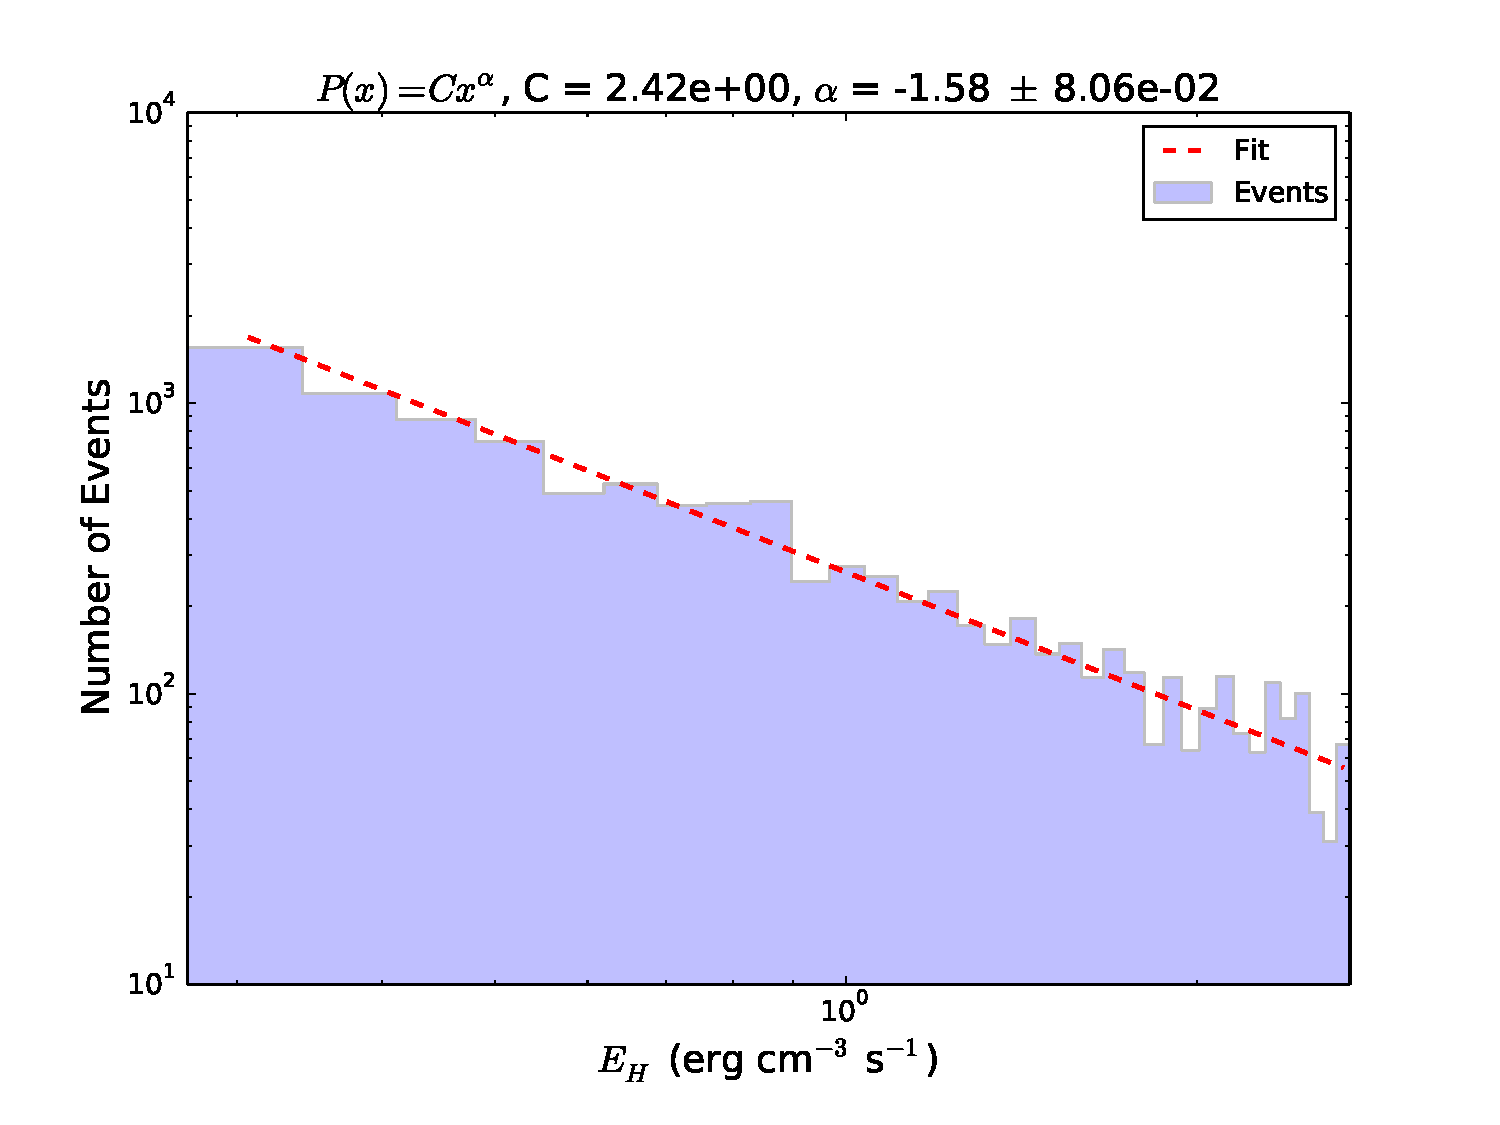
\includegraphics[width=0.85\textwidth]{figures/event_dist.pdf}
	\caption{Distribution of event energies for $L=40$ Mm, $\alpha=-1.5$, $T_N=5000$ s. While each run only includes $\sim16$ events, 625 runs are computed such that $N_{tot}\sim10^4$. The dashed red line shows the power-law fit to the resulting event distribution. The resulting $\alpha$ value from the fit is in good agreement with the specified value.}
	\label{fig:event_dist}
\end{figure}
%
\par Thus far, $T_N$ and $H_i$ have been treated independently. However, as discussed in \ref{subsec:dc_heating}, the twisted and stressed coronal field is thought to contribute to the supposed bursty heating of the corona. Following \citet{cargill_active_2014}, a model in which $Q_i\propto T_{N,i}^b$ is considered, where $Q_i,T_{N,i}$ are the total energy and waiting time following the $i$th event and $b=1,2$. The reasoning for such an expression is as follows. Bursty, nanoflare heating is thought to arise from the stressing and subsequent relaxation of the field. If a sufficient amount of time has elapsed since the last energy release event, the field will have had enough time to ``wind up'' such that the subsequent energy release is large. Conversely, if only a small amount of time has elapsed since the last event, the field will have not had time to become as stressed, resulting in a lower energy event. Thus, this scaling provides a way to incorporate a more realistic heating function into a hydrodynamic model which cannot self-consistently determine the heat input based on the evolving magnetic field. Fig. \ref{fig:heating_funcs} shows the various heating functions used for a variety of $T_N$ values.
%
\begin{figure}
	\centering
	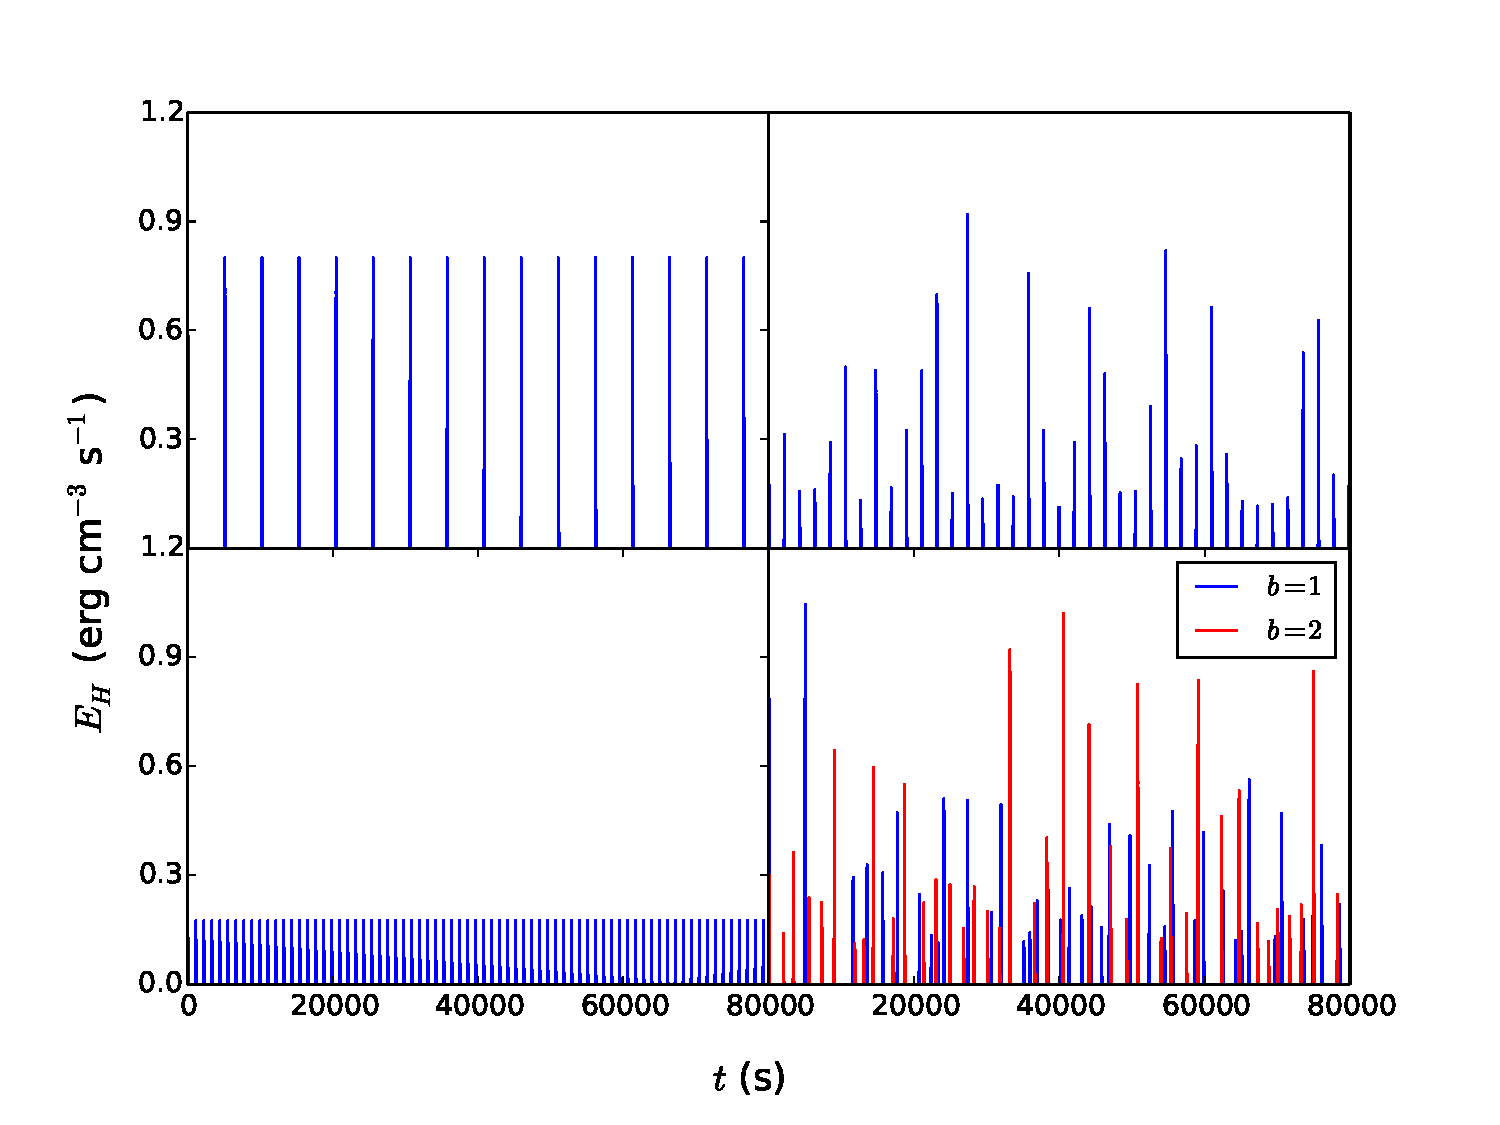
\includegraphics[width=0.85\textwidth]{figures/heating_functions.pdf}
	\caption{All heating functions are for $L=40$ Mm. Starting counter-clockwise from the bottom left: uniform heating amplitudes for $T_N=1000$ s; uniform heating amplitudes for $T_N=5000$ s; power-law distributed heating amplitudes for $\alpha=-1.5$, $T_N=2000$ s; power-law distributed amplitudes for $\alpha=-1.5$ where the wait times depend on the event energies and the mean wait time for both $b$ values is $\langle T_N\rangle=2000$ s.}
	\label{fig:heating_funcs}
\end{figure}
%
\section{Electron Heating}
\label{sec:electron_heating}
%
\hl{For each section, show L=40, all alpha, b=1,2}
\section{Ion Heating}
\label{sec:ion_heating}
%
\section{Single-fluid Comparisons}
\label{sec:single_fluid}